\documentclass[tikz, border=15pt]{standalone}
\usetikzlibrary{positioning}
\usepackage{tkz-graph}
\begin{document}
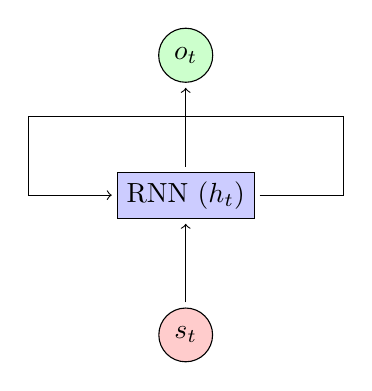
\begin{tikzpicture}

\node[draw, outer sep=2, circle, fill=red!20] (s_t) {$s_t$};
\node[draw, align=center, outer sep=2, fill=blue!20] (unit_t) [above=of s_t] {RNN ($h_t$)};
\node[draw, outer sep=2, circle, fill=green!20] (o_t) [above=of unit_t] {$o_t$};

\path[->] (s_t) edge (unit_t);
\path[->] (unit_t) edge (o_t);
\path[draw, style=->] (unit_t)  -- +(2, 0) -- +(2, 1) -- +(-2, 1) -- +(-2, 0) -- (unit_t);

\end{tikzpicture}
\end{document}